% Offizielle Beispieldatei für beamer-Vorlage aus tubslatex Version 0.3alpha2
\documentclass[fleqn,11pt]{beamer}

\usepackage[ngerman]{babel}
\usepackage[utf8x]{inputenc}
\usepackage{graphicx}
\usepackage{eurosym} % Für die Hardwarepreise
\usepackage{textpos}  % Für Grafikpositionierung
\usetheme[%
  %cmyk,%<rgbprint>,          Auswahl des Farbmodells
  blue,%<orange/green/violet> Auswahl des Sekundärfarbklangs
  dark,%<light,medium>        Auswahl der Helligkeit
  %colorhead,%    Farbig hinterlegte Kopfleiste
  %colorfoot,%    Farbig hinterlegt Fußleiste auf Titelseite
  colorblocks,%   Blöcke Farbig hinterlegen
  %nopagenum,%    Keine Seitennumer in Fußzeile
  %nodate,%       Kein Datum in Fußleiste
  tocinheader,%   Inhaltsverzeichnis in Kopfleiste
  %tinytocinheader,% kleines Kopfleisten-Inhaltsverzeichnis
  %widetoc,%      breites Kopfleisten-Inhaltsverzeichnis
  %narrowtoc,%    schmales Kopfleisten-Inhaltsverzeichnis
  %nosubsectionsinheader,%  Keine subsections im Kopfleisten-Inhaltsverzeichnis
  %nologoinfoot,% Kein Logo im Fußbereich darstellen
  ]{tubs}

% Titelseite
\title{AIO - Akustische Indoor-Ortung \\(Zwischenpräsentation)}
\subtitle{Praktikum Wireless Sensor Networks - Team 4}
\author{Johannes Starosta, Lena Schimmel}
% Titelgrafik, automatisch beschnitten, Weitere Optionen: <scaled/cropx/cropy>
% \titlegraphic[cropped]{\includegraphics{infozentrum.jpg}}
\titlegraphic[scaled]{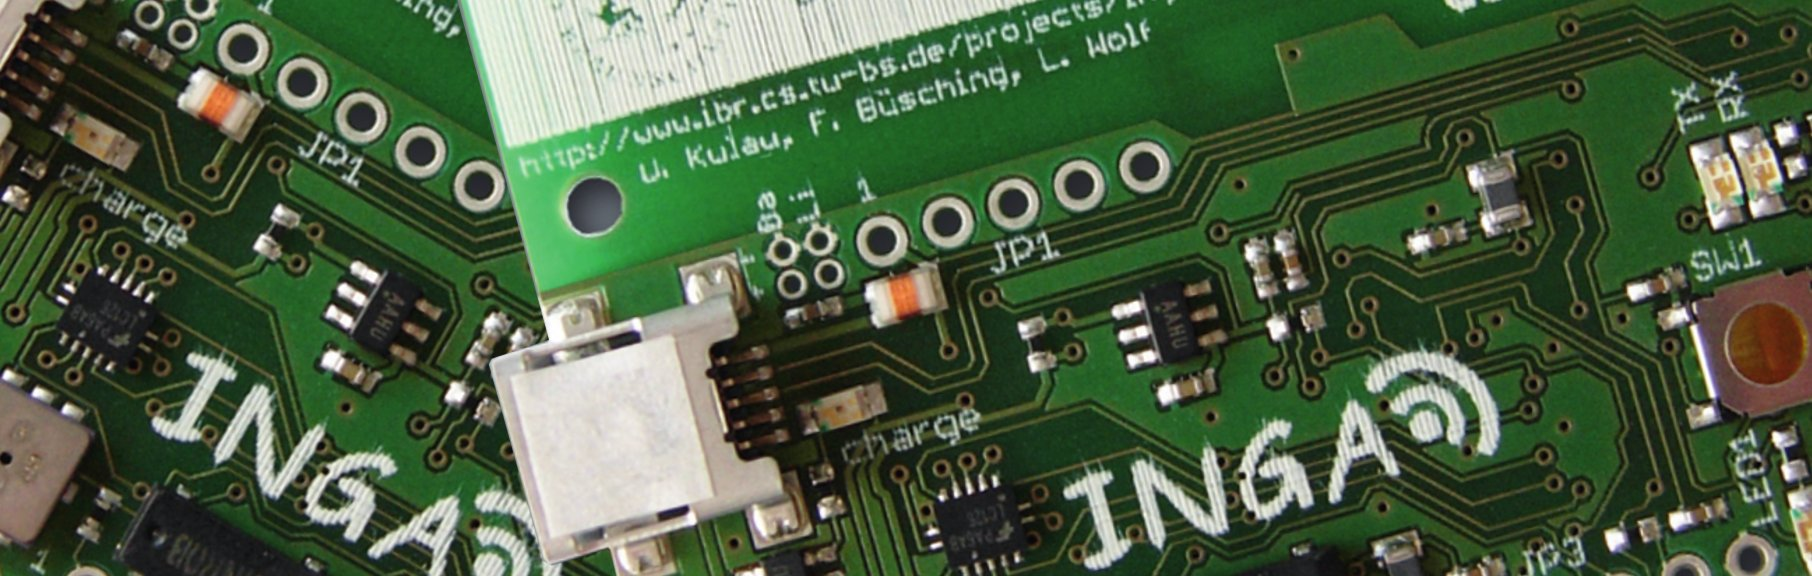
\includegraphics{titlepicture3.jpg}}

% Logo, dass auf Titelseiten oben rechts und auf Inthaltsseiten unten rechts
% dargestellt wird. Es wird jeweils automatisch skliert
\logo{
\includegraphics{ibr.jpg}}
%\logo{Institut für Unkreativität\\und Schreibschwäche}

\begin{document}

\begin{frame}[plain]
\titlepage
\end{frame}

\begin{frame}{Kurze Wiederholung: Idee}
	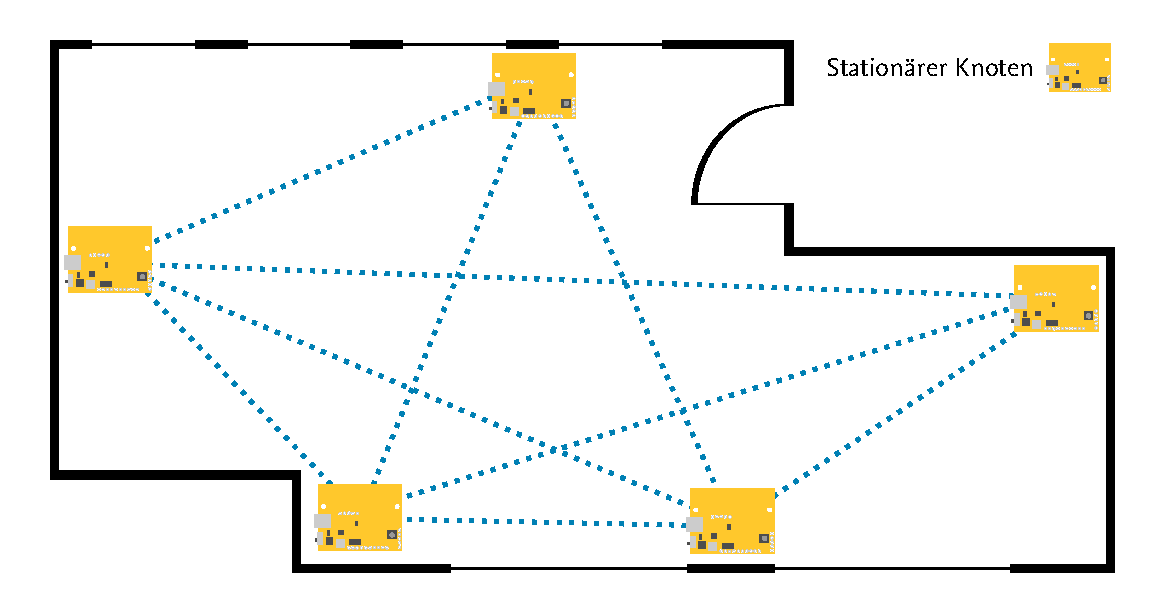
\includegraphics[width=0.48\textwidth]{room-2.pdf}
	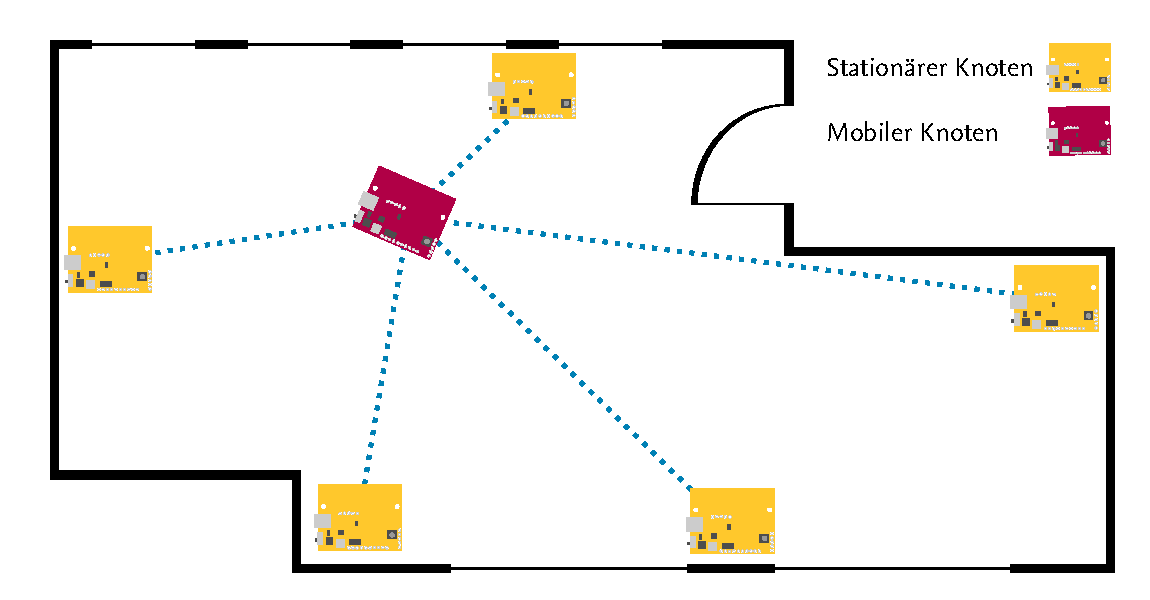
\includegraphics[width=0.48\textwidth]{room-3.pdf}

	\begin{itemize}
		\item Stationäre Knoten bestimmen ihre relative Lage zueinander
		\item Anschließend werden mobile Knoten geortet
		\item Beides geschieht über Laufzeitmessung akustischer Signale
	\end{itemize}
\end{frame}

\begin{frame}{Aktueller Status}
	\textbf{Was geht:}
	\begin{itemize}
		\item Die Arbeitsgrundlagen (Compiler, make, git)
		\item Zeitsynchronisation
		\item Analogsignale sampeln
	\end{itemize}
	
	\textbf{Was (noch) nicht geht:}
	\begin{itemize}
		\item Audio-Hardware
		\item Zuverlässiges Flashen der INGAs
		\item Thread-Scheduling
	\end{itemize}
\end{frame}

\begin{frame}{Programmierung (Joke)}
	\textit{(Joke...)}
\end{frame}

\begin{frame}{Hardware - Herausforderungen}
	\textbf{Versuche mit simpler Beschaltung nicht erfolgreich.}
	\begin{itemize}
		\item Signal Selbst zum Testen ungeeignet\\(Niedriger Gesamtpegel, hohes Rauschen)
		\item Standardhardware teilweise nur bis 10 kHz brauchbar und mit enormem Strom-/ Spannungsbedarf
		\item Menschen, die bis zu 19 kHz noch als störend wahrnehmen, Arbeit auf 20 kHz deshalb dringend nötig
	\end{itemize}
	
	\textbf{Deshalb: Komplexerer Hardwareentwurf nötig.}
\end{frame}

\begin{frame}{Hardware - Der Plan\textsuperscript{\small{TM}}}
%	\begin{floatingfigure}[l]{4cm}
 %   		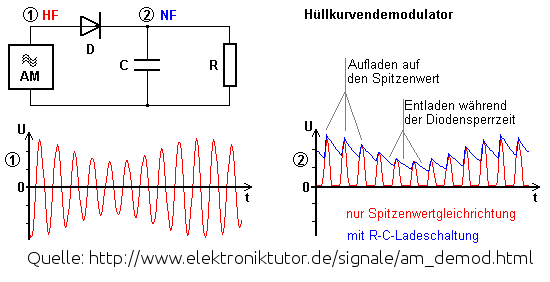
\includegraphics[width=0.5\textwidth]{amdemod.png}
%	\end{floatingigure}
\begin{textblock}{7}(7,0.3)
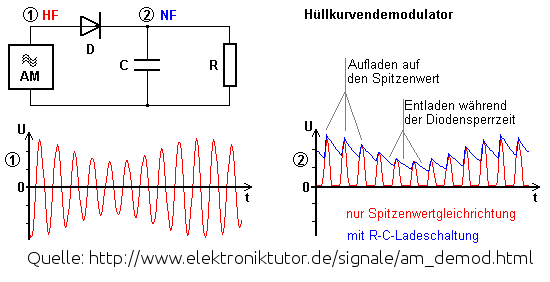
\includegraphics[width=1.0\textwidth]{amdemod.png}
\end{textblock}
\vspace*{1.2cm}
	\textbf{Hardware-Erweiterung}
	\begin{itemize}
		\item Zwei Audio-Kanäle
		\item Jeweils Ein- und Ausgabe
		\item Signalpipeline  bei der Eingabe:
		\begin{itemize}
			\item Elekret-Mikrofon mit Spannungseinspeisung
			\item Aktiver Bandpassfilter mit Verstärker in Multiple-Feedback-Topology \\(Frequenz über Potentiometer einstellbar) 
			\item Hüllkurvendemodulator (a.k.a. Spitzenwertgleichrichter)
			\item DA-Converter im ATmega1284P
		\end{itemize}
	\end{itemize}
	\textbf{Bauteilkosten:}\\ ca. \EUR{3} pro Board zzgl. \EUR{8} pro tatsächlich genutztem Kanal
\end{frame}


\begin{frame}{Hardware - Erster Entwurf}
	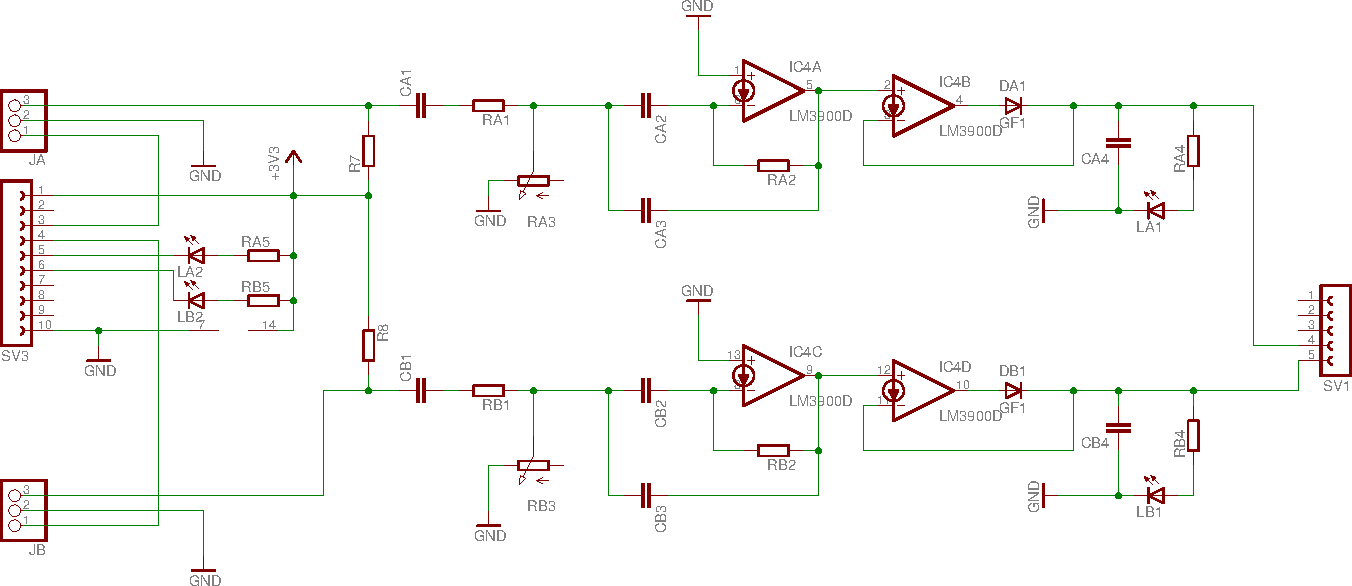
\includegraphics[width=1.0\textwidth]{AudioBoardSchema.pdf}
	
	Vorläufiger Schaltplan des Audio-Boards. Es fehlt die Verstärkung des Ausgabesignals und die Fingerprint-Funktionalität.
\end{frame}

\begin{frame}{Hardware - Erster Entwurf}
	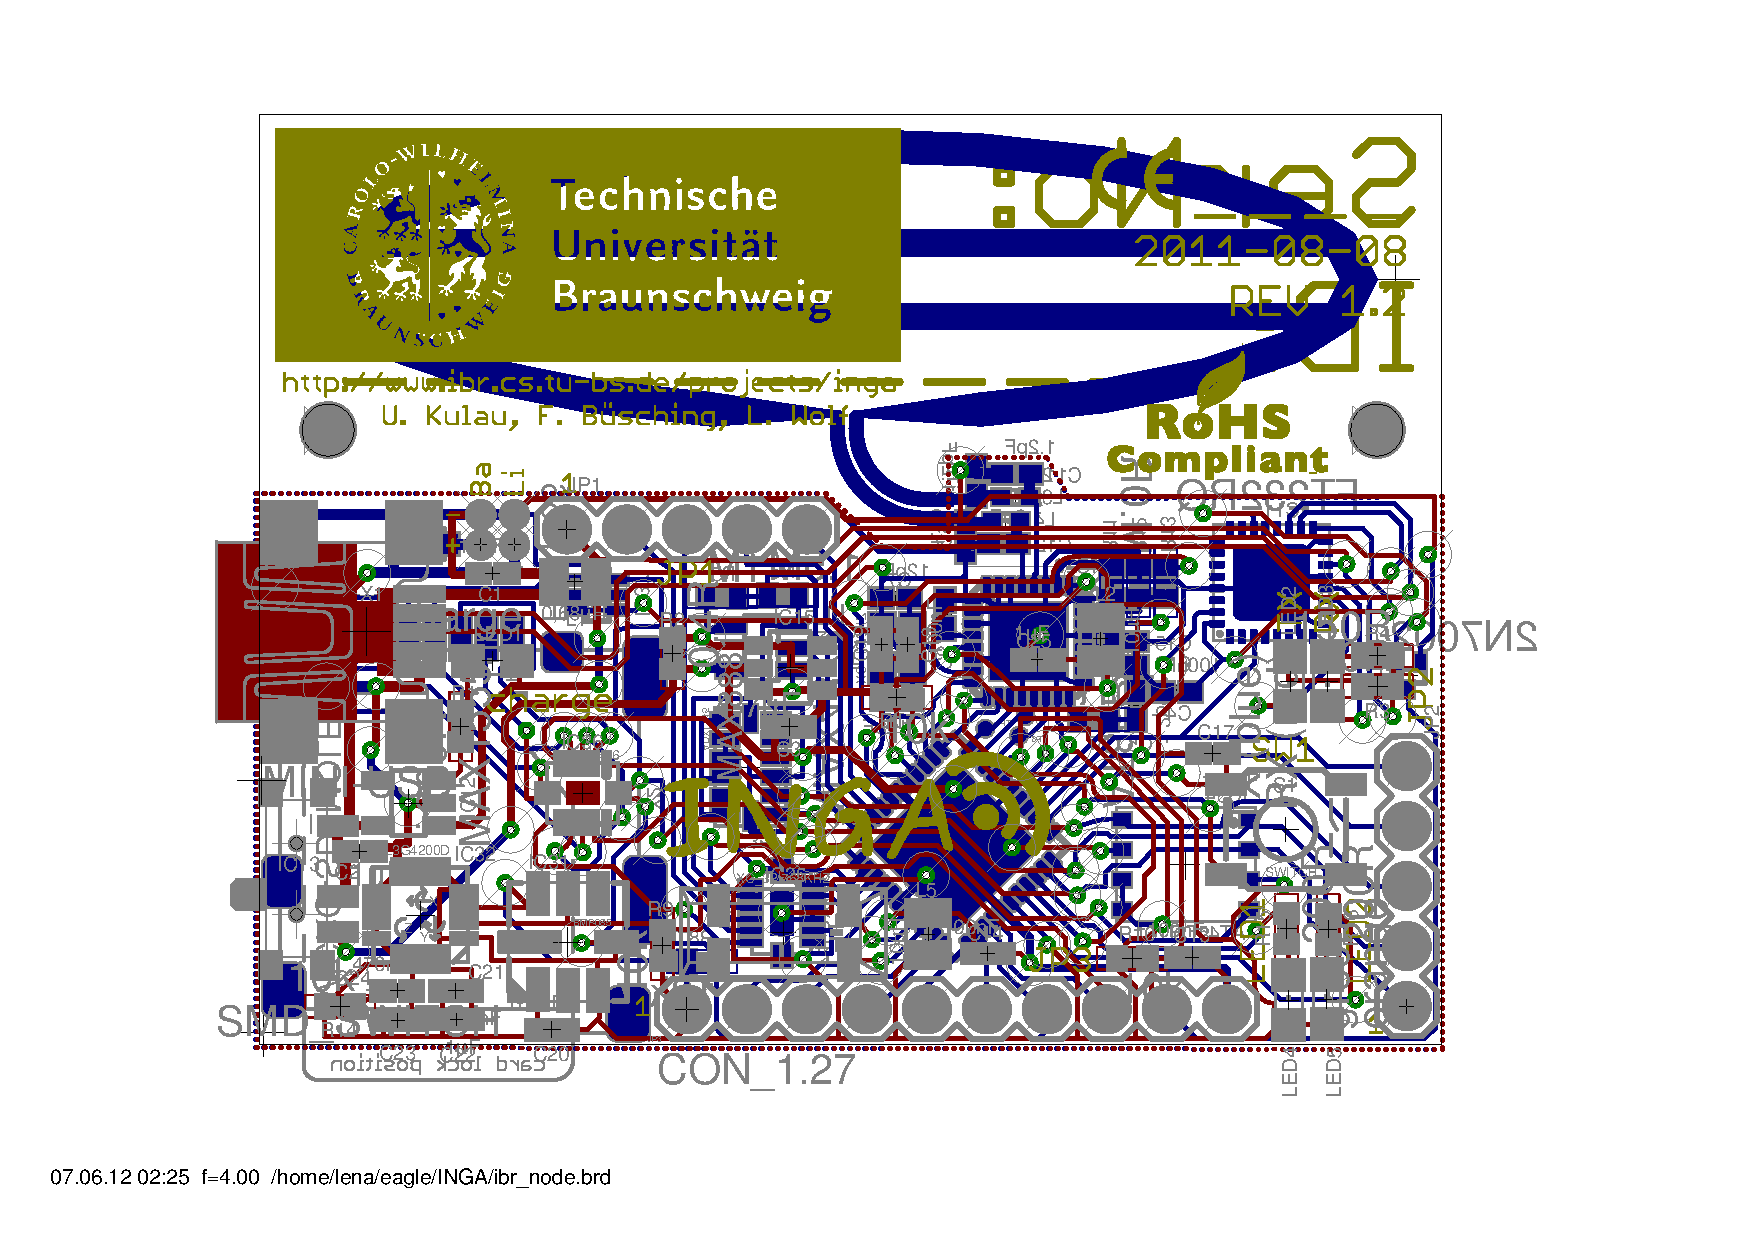
\includegraphics[width=0.55\textwidth]{ibr_node.pdf}
	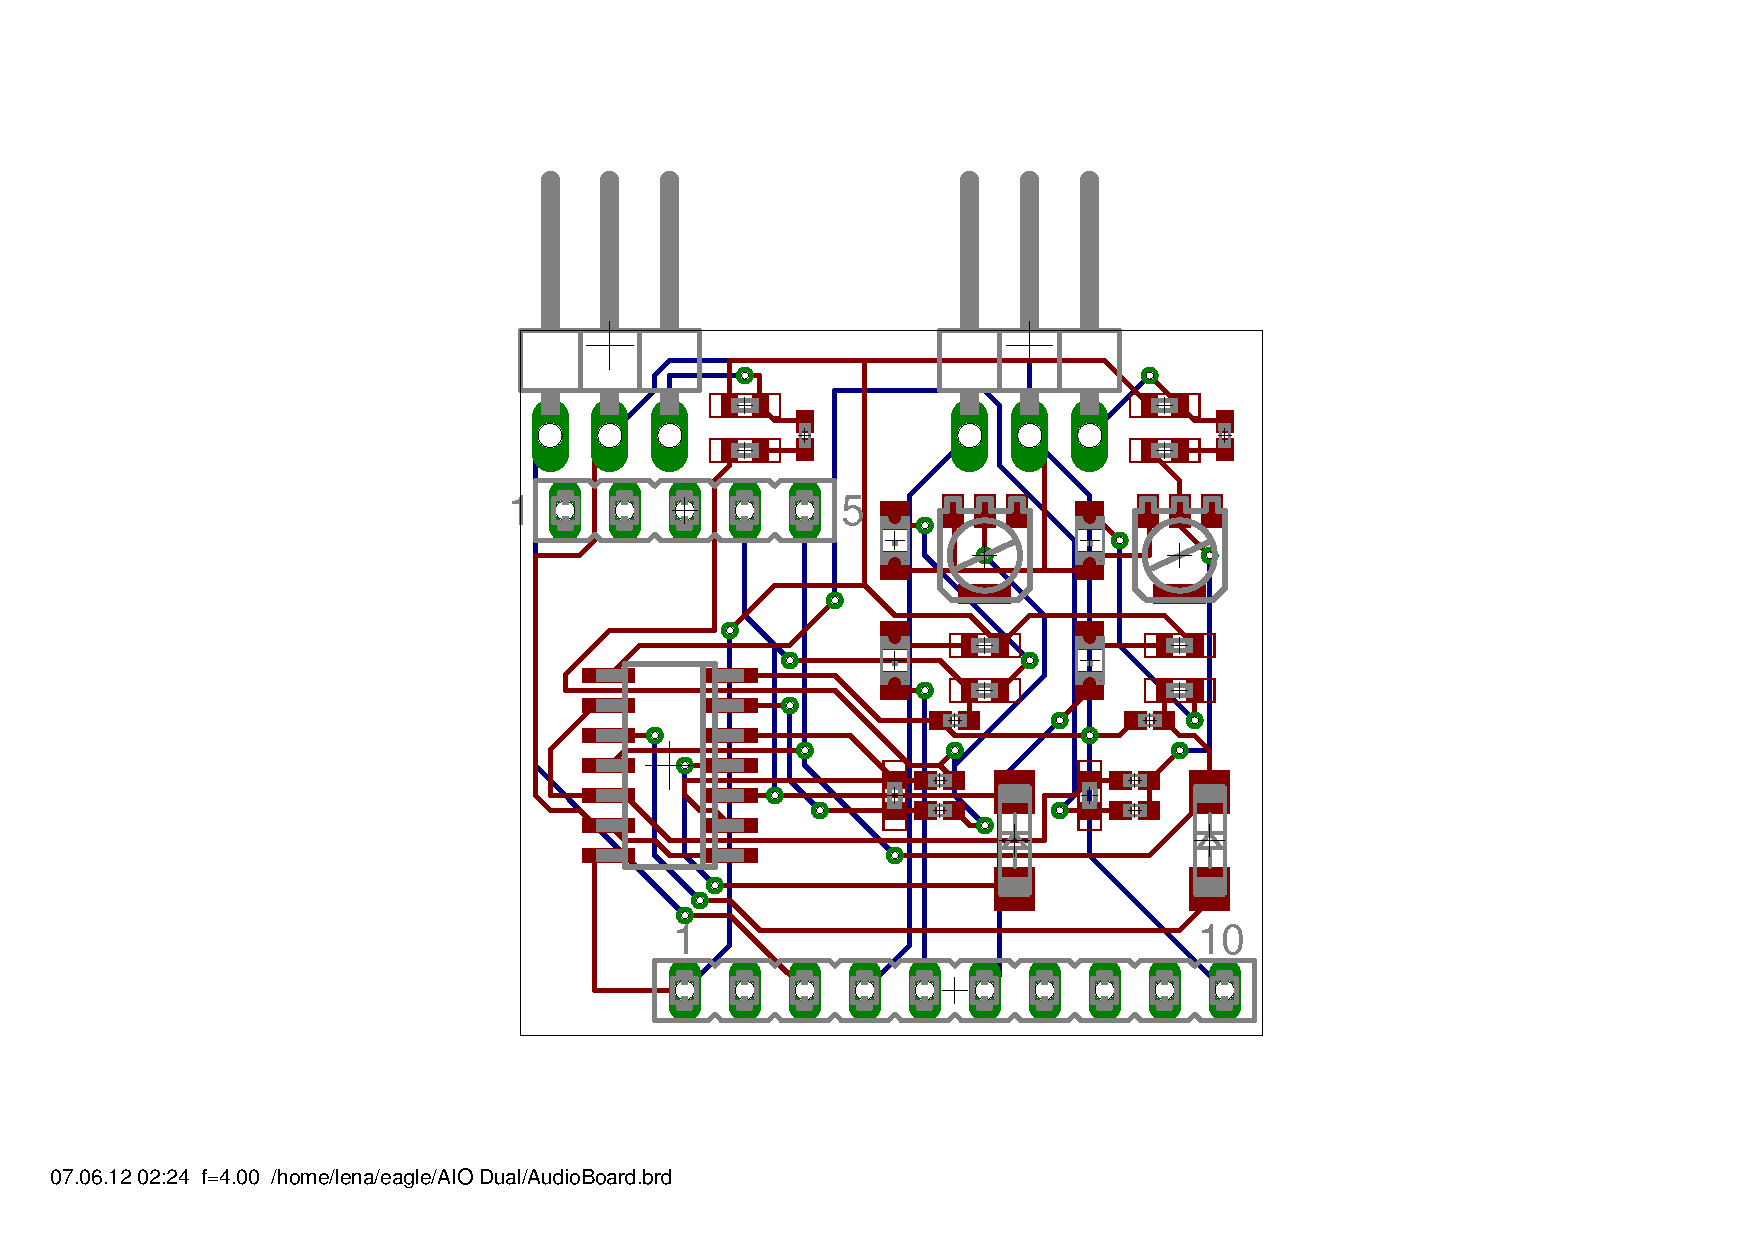
\includegraphics[width=0.55\textwidth]{AudioBoard.pdf}
	
	INGA und AudioBoard im gleichen Maßstab. Schalter und LEDs der INGA werden nicht verdeckt. Oben: gewinkelte Anschlüsse für Mikro und Lautsprecher.
\end{frame}


\begin{frame}{Was zu tun bleibt}
	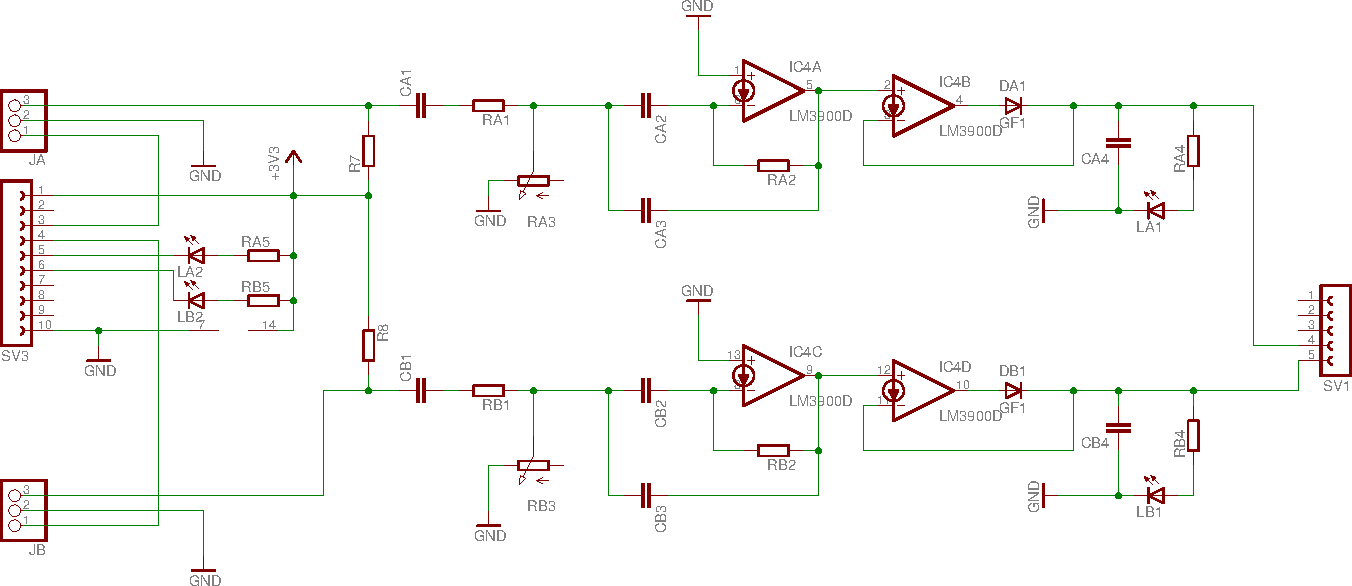
\includegraphics[width=1.0\textwidth]{AudioBoardSchema.pdf}
	
	Vorläufiger Schaltplan des Audio-Boards
\end{frame}

\begin{frame}{Hardware - Erster Entwurf}
	\begin{itemize}
		\item Programmieren
		\item 1-2 Prototypen der Hardware bauen
		\item Testen einer einzelnen Laufzeitmessung
		\item Kleinstserie der Hardware bauen
		\item Testen des Gesamtsystems
	\end{itemize}
\end{frame}

\end{document}
